\section{Metodo di bisezione}
\label{sec:metodoDiBisezione}
Riporto il codice di pagina 23:
\begin{lstlisting}
octave:12> p = poly([1.1*ones(1,20) pi])
p =
 Columns 1 through 6:
   1.0000e+00  -2.5142e+01   2.9902e+02  -2.2396e+03   1.1860e+04  -4.7254e+04
 Columns 7 through 12:
   1.4711e+05  -3.6678e+05   7.4461e+05  -1.2444e+06   1.7234e+06  -1.9847e+06
 Columns 13 through 18:
   1.9008e+06  -1.5096e+06   9.8794e+05  -5.2718e+05   2.2572e+05  -7.5702e+04
 Columns 19 through 22:
   1.9159e+04  -3.4410e+03   3.9100e+02  -2.1135e+01
octave:13> polyval(p,pi)
ans =  2.0207e-04
\end{lstlisting}
Lo scopo della funzione $poly(r)$ \`e quello di creare un vettore di coefficienti
di un polinomio $p$, tale che le radici di $p$ appartengono al vettore $r$ 
($poly: Root[] \rightarrow PolynomialCoefficient[]$).
Valutando quindi il polinomio in una sua radice (\emph{octave:13}) in aritmetica
esatta dovrei ottenere 0, mentre in aritmetica finita non \`e vero 
($p(\pi) = ans =  2.0207e-04 \not = 0$).

\begin{exercise}
Implementare il metodo di bisezione ed applicarlo alla funzione $\sin(x)$ 
con intervallo iniziale $[2, 5]$ ed una tollerenza $tolX = 10^{-14}$.
\end{exercise}
Per l'implementazione del codice vedere \nameref{sec:bisectionIterativeMethod}.
\begin{lstlisting}
octave:45> [x, i, imax, ascisse] = bisectionMethod('sin', 2, 5, e^-14)
x =  3.14159250259399e+00
i =  2.10000000000000e+01
imax =  2.20000000000000e+01
ascisse =
 Columns 1 through 3:
   3.50000000000000e+00   2.75000000000000e+00   3.12500000000000e+00
 Columns 4 through 6:
   3.31250000000000e+00   3.21875000000000e+00   3.17187500000000e+00
 Columns 7 through 9:
   3.14843750000000e+00   3.13671875000000e+00   3.14257812500000e+00
 Columns 10 through 12:
   3.13964843750000e+00   3.14111328125000e+00   3.14184570312500e+00
 Columns 13 through 15:
   3.14147949218750e+00   3.14166259765625e+00   3.14157104492188e+00
 Columns 16 through 18:
   3.14161682128906e+00   3.14159393310547e+00   3.14158248901367e+00
 Columns 19 through 21:
   3.14158821105957e+00   3.14159107208252e+00   3.14159250259399e+00
octave:46> xsin = min(ascisse):0.01:max(ascisse)
octave:47> ysin = feval('sin', xsin)
octave:48> [prepX, prepY] = prepareForPlottingMethodSegments(ascisse, 'sin')
octave:49> plot(xsin, ysin, "c", ascisse, feval('sin', ascisse), "b+", prepX, prepY, "r")
octave:50> print 'bisectionPlotOutput.tex' '-dTex' '-S800, 600'
\end{lstlisting}
Si raggiunge la tolleranza richiesta in 21 passi, uno in meno delle iterazioni
massime possibili. Questo l'output del comando \emph{octave:50}:
\begin{center}
% GNUPLOT: LaTeX picture with Postscript
\begingroup
  \makeatletter
  \providecommand\color[2][]{%
    \GenericError{(gnuplot) \space\space\space\@spaces}{%
      Package color not loaded in conjunction with
      terminal option `colourtext'%
    }{See the gnuplot documentation for explanation.%
    }{Either use 'blacktext' in gnuplot or load the package
      color.sty in LaTeX.}%
    \renewcommand\color[2][]{}%
  }%
  \providecommand\includegraphics[2][]{%
    \GenericError{(gnuplot) \space\space\space\@spaces}{%
      Package graphicx or graphics not loaded%
    }{See the gnuplot documentation for explanation.%
    }{The gnuplot epslatex terminal needs graphicx.sty or graphics.sty.}%
    \renewcommand\includegraphics[2][]{}%
  }%
  \providecommand\rotatebox[2]{#2}%
  \@ifundefined{ifGPcolor}{%
    \newif\ifGPcolor
    \GPcolortrue
  }{}%
  \@ifundefined{ifGPblacktext}{%
    \newif\ifGPblacktext
    \GPblacktexttrue
  }{}%
  % define a \g@addto@macro without @ in the name:
  \let\gplgaddtomacro\g@addto@macro
  % define empty templates for all commands taking text:
  \gdef\gplbacktext{}%
  \gdef\gplfronttext{}%
  \makeatother
  \ifGPblacktext
    % no textcolor at all
    \def\colorrgb#1{}%
    \def\colorgray#1{}%
  \else
    % gray or color?
    \ifGPcolor
      \def\colorrgb#1{\color[rgb]{#1}}%
      \def\colorgray#1{\color[gray]{#1}}%
      \expandafter\def\csname LTw\endcsname{\color{white}}%
      \expandafter\def\csname LTb\endcsname{\color{black}}%
      \expandafter\def\csname LTa\endcsname{\color{black}}%
      \expandafter\def\csname LT0\endcsname{\color[rgb]{1,0,0}}%
      \expandafter\def\csname LT1\endcsname{\color[rgb]{0,1,0}}%
      \expandafter\def\csname LT2\endcsname{\color[rgb]{0,0,1}}%
      \expandafter\def\csname LT3\endcsname{\color[rgb]{1,0,1}}%
      \expandafter\def\csname LT4\endcsname{\color[rgb]{0,1,1}}%
      \expandafter\def\csname LT5\endcsname{\color[rgb]{1,1,0}}%
      \expandafter\def\csname LT6\endcsname{\color[rgb]{0,0,0}}%
      \expandafter\def\csname LT7\endcsname{\color[rgb]{1,0.3,0}}%
      \expandafter\def\csname LT8\endcsname{\color[rgb]{0.5,0.5,0.5}}%
    \else
      % gray
      \def\colorrgb#1{\color{black}}%
      \def\colorgray#1{\color[gray]{#1}}%
      \expandafter\def\csname LTw\endcsname{\color{white}}%
      \expandafter\def\csname LTb\endcsname{\color{black}}%
      \expandafter\def\csname LTa\endcsname{\color{black}}%
      \expandafter\def\csname LT0\endcsname{\color{black}}%
      \expandafter\def\csname LT1\endcsname{\color{black}}%
      \expandafter\def\csname LT2\endcsname{\color{black}}%
      \expandafter\def\csname LT3\endcsname{\color{black}}%
      \expandafter\def\csname LT4\endcsname{\color{black}}%
      \expandafter\def\csname LT5\endcsname{\color{black}}%
      \expandafter\def\csname LT6\endcsname{\color{black}}%
      \expandafter\def\csname LT7\endcsname{\color{black}}%
      \expandafter\def\csname LT8\endcsname{\color{black}}%
    \fi
  \fi
  \setlength{\unitlength}{0.0500bp}%
  \begin{picture}(7680.00,5760.00)%
    \gplgaddtomacro\gplbacktext{%
      \colorrgb{0.00,0.00,0.00}%
      \put(866,634){\makebox(0,0)[r]{\strut{}-0.4}}%
      \colorrgb{0.00,0.00,0.00}%
      \put(866,1221){\makebox(0,0)[r]{\strut{}-0.3}}%
      \colorrgb{0.00,0.00,0.00}%
      \put(866,1807){\makebox(0,0)[r]{\strut{}-0.2}}%
      \colorrgb{0.00,0.00,0.00}%
      \put(866,2394){\makebox(0,0)[r]{\strut{}-0.1}}%
      \colorrgb{0.00,0.00,0.00}%
      \put(866,2981){\makebox(0,0)[r]{\strut{}0}}%
      \colorrgb{0.00,0.00,0.00}%
      \put(866,3567){\makebox(0,0)[r]{\strut{}0.1}}%
      \colorrgb{0.00,0.00,0.00}%
      \put(866,4154){\makebox(0,0)[r]{\strut{}0.2}}%
      \colorrgb{0.00,0.00,0.00}%
      \put(866,4740){\makebox(0,0)[r]{\strut{}0.3}}%
      \colorrgb{0.00,0.00,0.00}%
      \put(866,5327){\makebox(0,0)[r]{\strut{}0.4}}%
      \colorrgb{0.00,0.00,0.00}%
      \put(998,414){\makebox(0,0){\strut{}2.6}}%
      \colorrgb{0.00,0.00,0.00}%
      \put(2188,414){\makebox(0,0){\strut{}2.8}}%
      \colorrgb{0.00,0.00,0.00}%
      \put(3379,414){\makebox(0,0){\strut{}3}}%
      \colorrgb{0.00,0.00,0.00}%
      \put(4569,414){\makebox(0,0){\strut{}3.2}}%
      \colorrgb{0.00,0.00,0.00}%
      \put(5760,414){\makebox(0,0){\strut{}3.4}}%
      \colorrgb{0.00,0.00,0.00}%
      \put(6950,414){\makebox(0,0){\strut{}3.6}}%
    }%
    \gplgaddtomacro\gplfronttext{%
    }%
    \gplbacktext
    \put(0,0){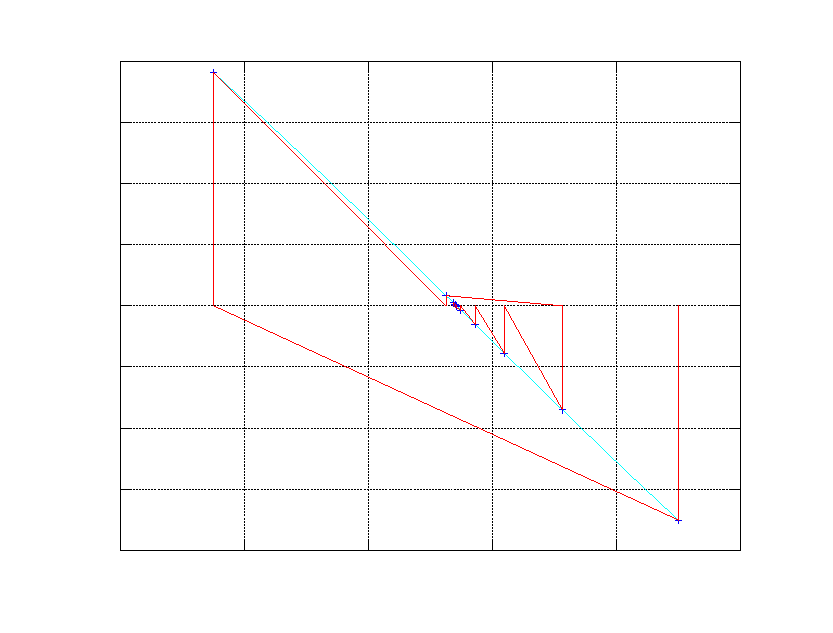
\includegraphics{RadiciEquazione/bisectionPlotOutput}}%
    \gplfronttext
  \end{picture}%
\endgroup

\end{center}
Ho rappresentato nel grafico tre curve: 
\begin{itemize}
  \item con la curva cyan la rappresentazione della funzione $\sin(x)$
  \item con la curva blu, composta da pochi simboli '$+$', i punti
  calcolati dal metodo di bisezione per convergere allo zero $\pi$
  \item con la curva rossa il metodo di bisezione per visualizzare
  la sequenza con cui si procede per convergere alla soluzione.
\end{itemize}

\begin{exercise}
Implementare il metodo di bisezione ed applicarlo alla funzione $\sin(x)$ 
con intervallo iniziale $[-0.1, 7]$, in modo da avere due zeri nell'
intervallo di confidenza, ed una tollerenza $tolX = 10^{-14}$.
\end{exercise}
Per l'implementazione del codice vedere \nameref{sec:bisectionIterativeMethod}.
\begin{lstlisting}
octave:51> [x, i, imax, ascisse] = bisectionMethod('sin', -0.1, 7, e^-14)
x =  6.28318557739258e+00
i =  1.70000000000000e+01
imax =  2.40000000000000e+01
ascisse =
 Columns 1 through 3:
   3.45000000000000e+00   5.22500000000000e+00   6.11250000000000e+00
 Columns 4 through 6:
   6.55625000000000e+00   6.33437500000000e+00   6.22343750000000e+00
 Columns 7 through 9:
   6.27890625000000e+00   6.30664062500000e+00   6.29277343750000e+00
 Columns 10 through 12:
   6.28583984375000e+00   6.28237304687500e+00   6.28410644531250e+00
 Columns 13 through 15:
   6.28323974609375e+00   6.28280639648438e+00   6.28302307128906e+00
 Columns 16 and 17:
   6.28313140869141e+00   6.28318557739258e+00
octave:52> xsin = min(ascisse):0.01:max(ascisse)
octave:53> ysin = feval('sin', xsin)
octave:54> plot(xsin, ysin, ascisse, feval('sin', ascisse), '+')
octave:55> print 'bisectionWithTwoRootsPlotOutput.tex' '-dTex' '-S700, 500'
\end{lstlisting}
Si raggiunge la tolleranza richiesta in 17 passi, sette in meno delle iterazioni massime possibili. Questo l'output del comando \emph{octave:55}:
\begin{center}
% GNUPLOT: LaTeX picture with Postscript
\begingroup
  \makeatletter
  \providecommand\color[2][]{%
    \GenericError{(gnuplot) \space\space\space\@spaces}{%
      Package color not loaded in conjunction with
      terminal option `colourtext'%
    }{See the gnuplot documentation for explanation.%
    }{Either use 'blacktext' in gnuplot or load the package
      color.sty in LaTeX.}%
    \renewcommand\color[2][]{}%
  }%
  \providecommand\includegraphics[2][]{%
    \GenericError{(gnuplot) \space\space\space\@spaces}{%
      Package graphicx or graphics not loaded%
    }{See the gnuplot documentation for explanation.%
    }{The gnuplot epslatex terminal needs graphicx.sty or graphics.sty.}%
    \renewcommand\includegraphics[2][]{}%
  }%
  \providecommand\rotatebox[2]{#2}%
  \@ifundefined{ifGPcolor}{%
    \newif\ifGPcolor
    \GPcolortrue
  }{}%
  \@ifundefined{ifGPblacktext}{%
    \newif\ifGPblacktext
    \GPblacktexttrue
  }{}%
  % define a \g@addto@macro without @ in the name:
  \let\gplgaddtomacro\g@addto@macro
  % define empty templates for all commands taking text:
  \gdef\gplbacktext{}%
  \gdef\gplfronttext{}%
  \makeatother
  \ifGPblacktext
    % no textcolor at all
    \def\colorrgb#1{}%
    \def\colorgray#1{}%
  \else
    % gray or color?
    \ifGPcolor
      \def\colorrgb#1{\color[rgb]{#1}}%
      \def\colorgray#1{\color[gray]{#1}}%
      \expandafter\def\csname LTw\endcsname{\color{white}}%
      \expandafter\def\csname LTb\endcsname{\color{black}}%
      \expandafter\def\csname LTa\endcsname{\color{black}}%
      \expandafter\def\csname LT0\endcsname{\color[rgb]{1,0,0}}%
      \expandafter\def\csname LT1\endcsname{\color[rgb]{0,1,0}}%
      \expandafter\def\csname LT2\endcsname{\color[rgb]{0,0,1}}%
      \expandafter\def\csname LT3\endcsname{\color[rgb]{1,0,1}}%
      \expandafter\def\csname LT4\endcsname{\color[rgb]{0,1,1}}%
      \expandafter\def\csname LT5\endcsname{\color[rgb]{1,1,0}}%
      \expandafter\def\csname LT6\endcsname{\color[rgb]{0,0,0}}%
      \expandafter\def\csname LT7\endcsname{\color[rgb]{1,0.3,0}}%
      \expandafter\def\csname LT8\endcsname{\color[rgb]{0.5,0.5,0.5}}%
    \else
      % gray
      \def\colorrgb#1{\color{black}}%
      \def\colorgray#1{\color[gray]{#1}}%
      \expandafter\def\csname LTw\endcsname{\color{white}}%
      \expandafter\def\csname LTb\endcsname{\color{black}}%
      \expandafter\def\csname LTa\endcsname{\color{black}}%
      \expandafter\def\csname LT0\endcsname{\color{black}}%
      \expandafter\def\csname LT1\endcsname{\color{black}}%
      \expandafter\def\csname LT2\endcsname{\color{black}}%
      \expandafter\def\csname LT3\endcsname{\color{black}}%
      \expandafter\def\csname LT4\endcsname{\color{black}}%
      \expandafter\def\csname LT5\endcsname{\color{black}}%
      \expandafter\def\csname LT6\endcsname{\color{black}}%
      \expandafter\def\csname LT7\endcsname{\color{black}}%
      \expandafter\def\csname LT8\endcsname{\color{black}}%
    \fi
  \fi
  \setlength{\unitlength}{0.0500bp}%
  \begin{picture}(7680.00,5760.00)%
    \gplgaddtomacro\gplbacktext{%
      \colorrgb{0.00,0.00,0.00}%
      \put(866,634){\makebox(0,0)[r]{\strut{}-1}}%
      \colorrgb{0.00,0.00,0.00}%
      \put(866,1304){\makebox(0,0)[r]{\strut{}-0.8}}%
      \colorrgb{0.00,0.00,0.00}%
      \put(866,1975){\makebox(0,0)[r]{\strut{}-0.6}}%
      \colorrgb{0.00,0.00,0.00}%
      \put(866,2645){\makebox(0,0)[r]{\strut{}-0.4}}%
      \colorrgb{0.00,0.00,0.00}%
      \put(866,3316){\makebox(0,0)[r]{\strut{}-0.2}}%
      \colorrgb{0.00,0.00,0.00}%
      \put(866,3986){\makebox(0,0)[r]{\strut{}0}}%
      \colorrgb{0.00,0.00,0.00}%
      \put(866,4657){\makebox(0,0)[r]{\strut{}0.2}}%
      \colorrgb{0.00,0.00,0.00}%
      \put(866,5327){\makebox(0,0)[r]{\strut{}0.4}}%
      \colorrgb{0.00,0.00,0.00}%
      \put(998,414){\makebox(0,0){\strut{}3}}%
      \colorrgb{0.00,0.00,0.00}%
      \put(1742,414){\makebox(0,0){\strut{}3.5}}%
      \colorrgb{0.00,0.00,0.00}%
      \put(2486,414){\makebox(0,0){\strut{}4}}%
      \colorrgb{0.00,0.00,0.00}%
      \put(3230,414){\makebox(0,0){\strut{}4.5}}%
      \colorrgb{0.00,0.00,0.00}%
      \put(3974,414){\makebox(0,0){\strut{}5}}%
      \colorrgb{0.00,0.00,0.00}%
      \put(4718,414){\makebox(0,0){\strut{}5.5}}%
      \colorrgb{0.00,0.00,0.00}%
      \put(5462,414){\makebox(0,0){\strut{}6}}%
      \colorrgb{0.00,0.00,0.00}%
      \put(6206,414){\makebox(0,0){\strut{}6.5}}%
      \colorrgb{0.00,0.00,0.00}%
      \put(6950,414){\makebox(0,0){\strut{}7}}%
    }%
    \gplgaddtomacro\gplfronttext{%
    }%
    \gplbacktext
    \put(0,0){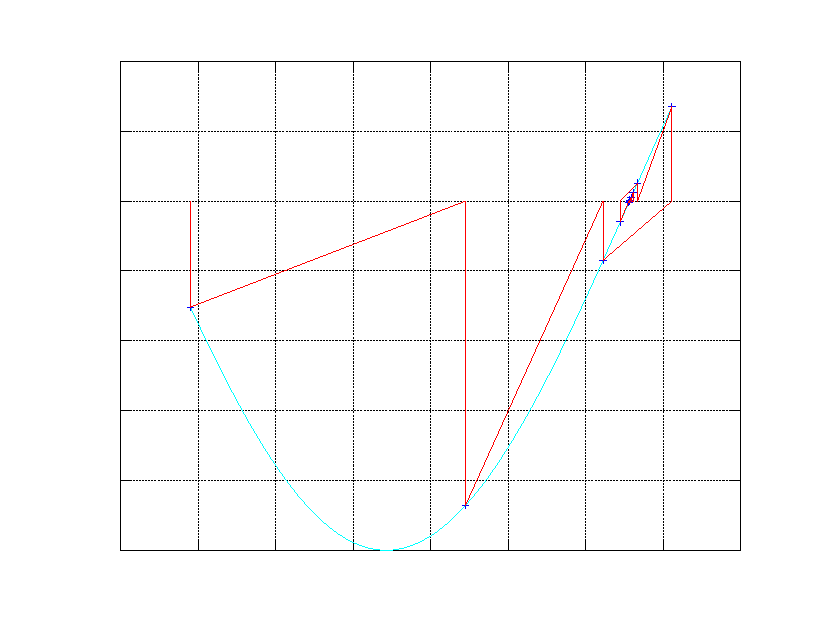
\includegraphics{RadiciEquazione/bisectionWithTwoRootsPlotOutput}}%
    \gplfronttext
  \end{picture}%
\endgroup

\end{center}
Ho rappresentato nel grafico tre curve: 
\begin{itemize}
  \item con la curva cyan la rappresentazione della funzione $\sin(x)$
  \item con la curva blu, composta da pochi simboli '$+$', i punti
  calcolati dal metodo di bisezione per convergere allo zero $2\pi$
  \item con la curva rossa il metodo di bisezione per visualizzare
  la sequenza con cui si procede per convergere alla soluzione.
\end{itemize}

Da questo esercizio si vede che il metodo di bisezione converge comunque
ad una radice, anche nel caso in cui nell'intervallo di confidenza ci sono
pi\`u zeri della funzione.




